\documentclass[border=6pt]{standalone}
\usepackage{tikz}
\usetikzlibrary{arrows.meta,backgrounds}

\begin{document}
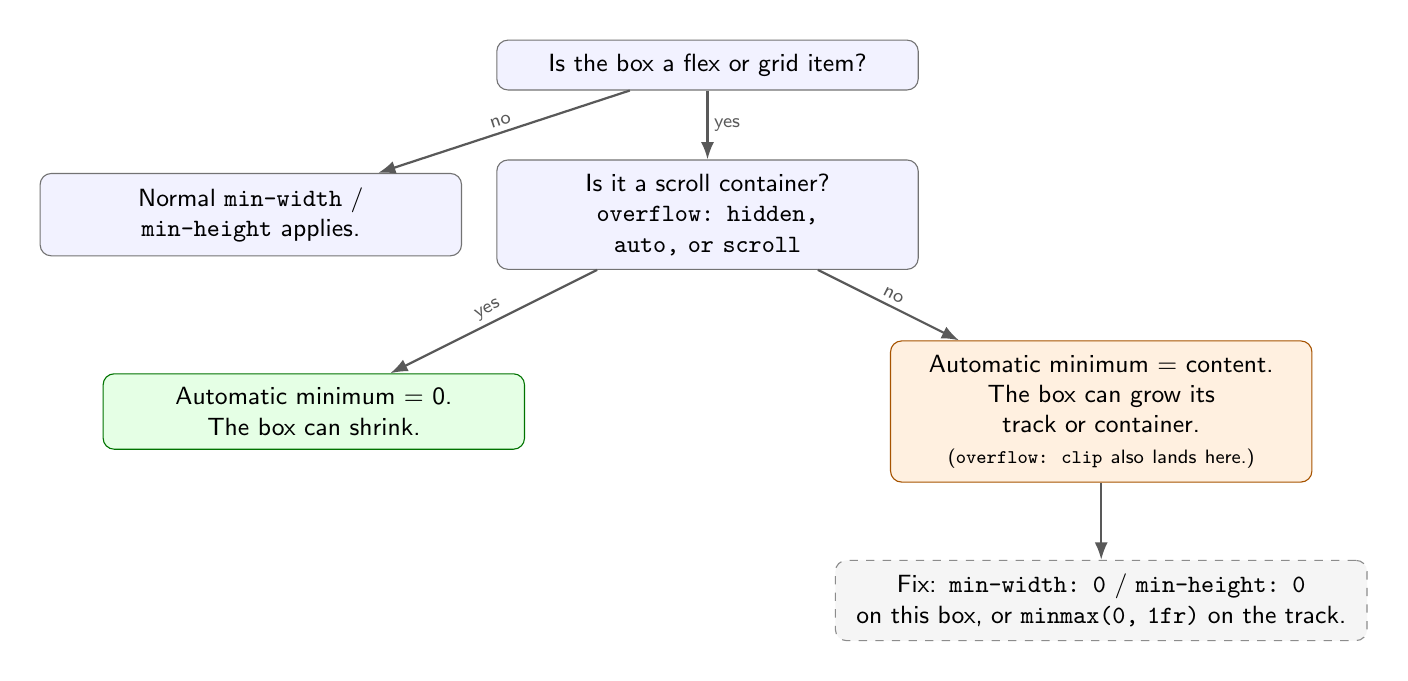
\begin{tikzpicture}[
  font=\sffamily\small,
  show background rectangle,
  background rectangle/.style={fill=white},
  box/.style={rectangle, rounded corners=4pt, draw=black!55, fill=blue!5,
    text width=5.0cm, align=center, inner sep=5pt},
  good/.style={box, fill=green!10, draw=green!45!black},
  bad/.style={box, fill=orange!12, draw=orange!65!black},
  action/.style={box, text width=6.4cm, fill=gray!8, draw=black!45, dashed},
  arrow/.style={-{Latex[length=2.2mm]}, thick, draw=black!65},
  branch/.style={font=\sffamily\scriptsize, text=black!65, inner sep=2pt}
]
  \node[box] (start) at (0,0) {Is the box a flex or grid item?};
  \node[box] (normal) at (-5.8,-1.9) {Normal \texttt{min-width} /\\\texttt{min-height} applies.};
  \node[box] (scroll) at (0,-1.9) {Is it a scroll container?\\\texttt{overflow: hidden,}\\\texttt{auto, or scroll}};
  \node[good] (zero) at (-5.0,-4.4) {Automatic minimum = 0.\\The box can shrink.};
  \node[bad] (content) at (5.0,-4.4) {Automatic minimum = content.\\The box can grow its track or container.\\{\scriptsize(\texttt{overflow: clip} also lands here.)}};
  \node[action] (fix) at (5.0,-6.8) {Fix: \texttt{min-width: 0} / \texttt{min-height: 0}\\on this box, or \texttt{minmax(0, 1fr)} on the track.};

  \draw[arrow] (start) -- (normal) node[midway, above, sloped, branch] {no};
  \draw[arrow] (start) -- (scroll) node[midway, right, branch] {yes};
  \draw[arrow] (scroll) -- (zero) node[midway, above, sloped, branch] {yes};
  \draw[arrow] (scroll) -- (content) node[midway, above, sloped, branch] {no};
  \draw[arrow] (content) -- (fix);
\end{tikzpicture}
\end{document}
